\documentclass[a4paper]{article}
\usepackage{amsmath}
\usepackage{amsfonts}
\usepackage[affil-it]{authblk}
\usepackage[backend=bibtex,style=numeric]{biblatex}

\usepackage{geometry}
\geometry{margin=1.5cm, vmargin={0pt,1cm}}
\setlength{\topmargin}{-1cm}
\setlength{\paperheight}{29.7cm}
\setlength{\textheight}{25.3cm}
\setlength{\parindent}{0pt}

\addbibresource{references.bib}

\usepackage{pgfplots}
\pgfplotsset{compat=1.16}

\usepackage{microtype}

\begin{document}
% =================================================
\title{Report For Ch2 Programming Hw}

\author{WangHao 3220103613
  \thanks{Electronic address: \texttt{3220103613@zju.edu.cn}}}
\affil{(Information and Computing Sciences, Class 2201), Zhejiang University }


\date{Due time: \today}

\maketitle






% ============================================
\section*{A: Design of Newton formula interpolation, Hermite problem interpolation and Bezier curve}



\section*{B.}

We use \texttt{class Interpolator\_N} to interpolate with Newton formula. 
We set the exact function of interpolator. 
Then we set the interpolating points and do interpolation. Repeated it 4 times, we get 4 interpolation polynomial.

\begin{flalign*}
  & p_1(x) = 1 - 0.0384615x^2 \\
  & p_3(x) = 1 - 0.171088x^2 + 0.00530504x^4 \\
  & p_5(x) = 1 - 0.351364x^2 + 0.0335319x^4 - 0.000840633x^6 \\
  & p_7(x) = 1 - 0.528121x^2 + 0.0981875x^4 - 0.00658016x^6 + 0.000137445x^8 
\end{flalign*}

Thus we can plot the polynomials against the exact function. It is presented below.

\begin{center}
  \begin{tikzpicture}
    \begin{axis}[
        xlabel=$x$,
        ylabel=$y$,
        domain=-5:5,
        samples=200,
        legend pos=outer north east,
        enlargelimits={abs=0.5},
        axis lines=middle,
        xtick={-5,-4,...,5},
        ytick={-1,-0.5,...,1},
        xmin=-5.5, xmax=5.5,
        ymin=-1.5, ymax=1.5,
    ]
    
    \addplot[blue, thick] {1/(1+x^2)};
    \addlegendentry{$f(x) = \frac{1}{1+x^2}$}
    
    \addplot[red, dashed] {1 - 0.0384615*x^2};
    \addlegendentry{$p_{n(=2)}(x)$}
    
    \addplot[green, dotted] {1 - 0.171088*x^2 + 0.00530504*x^4};
    \addlegendentry{$p_{n(=4)}(x)$}
    
    \addplot[orange, dashdotted] {1 - 0.351364*x^2 + 0.0335319*x^4 - 0.000840633*x^6};
    \addlegendentry{$p_{n(=6)}(x)$}
    
    \addplot[purple, densely dashed] {1 - 0.528121*x^2 + 0.0981875*x^4 - 0.00658016*x^6 + 0.000137445*x^8};
    \addlegendentry{$p_{n(=8)}(x)$}
    
    \end{axis}
  \end{tikzpicture}
\end{center}

It can be easily observed that 
as the number of interpolating points increases, 
the interpolation polynomial does not consistently converge to the original function at the ends of the interval, 
which is known as Runge phenomenon.

\section*{C.}

Like Problem b, 
We use \texttt{class Interpolator\_N} to interpolate with Newton formula. 
We set the exact function of interpolator. 
Then we set the interpolating points and do interpolation. Repeated it 4 times, we get 4 interpolation polynomial, 
which is presented in the output of the program.

Thus we can plot the polynomials against the exact function. It is presented below.

\begin{center}
  \begin{tikzpicture}
    \begin{axis}[
        xlabel=$x$,
        ylabel=$y$,
        domain=-1:1,
        samples=200,
        legend pos=outer north east,
        enlargelimits={abs=0.5},
        axis lines=middle,
        xtick={-1,-0.5,...,1},
        ytick={-1,-0.5,...,1},
        xmin=-1, xmax=1,
        ymin=-1.5, ymax=1.5,
    ]
    
    \addplot[blue, thick] {1/(1+25*x^2)};
    \addlegendentry{$f(x) = \frac{1}{1+25x^2}$}
    
    \addplot[red, dashed] {1 - 3.54298*x^2 + 2.7465*x^4};
    \addlegendentry{$p_{n(=5)}(x)$}
    
    \addplot[green, dotted] {0.730822 - 4.81162*x^2 + 3.06605e-14*x^3 + 12.6193*x^4 - 5.5704e-14*x^5 - 14.0024*x^6 + 9.10478e-14*x^7 + 5.51277*x^8 - 3.64196e-14*x^9};
    \addlegendentry{$p_{n(=10)}(x)$}
    
    \addplot[orange, dashdotted] {1 - 17.3641*x^2 + 149.027*x^4 + 3.69482e-13*x^5 - 646.864*x^6 + 1.76215e-12*x^7 + 1510.61*x^8 + 2.84217e-12*x^9 - 1927.18*x^10 - 9.09495e-13*x^11 + 1264.42*x^12 - 5.68434e-14*x^13 - 333.619*x^14};
    \addlegendentry{$p_{n(=15)}(x)$}
    
    \addplot[purple, densely dashed] {0.96241 - 16.5422*x^2 + 6.65006e-14*x^3 + 165.458*x^4 - 1.95768e-12*x^5 - 960.825*x^6 - 1.72285e-11*x^7 + 3379.02*x^8 - 7.60981e-11*x^9 - 7413.45*x^10 - 6.12795e-11*x^11 + 10195.5*x^12 - 1.17966e-10*x^13 - 8534.89*x^14 + 3.93281e-12*x^15 + 3973.16*x^16 - 1.66573e-11*x^17 - 788.326*x^18 + 3.19307e-12*x^19};
    \addlegendentry{$p_{n(=20)}(x)$}
    
    \end{axis}
  \end{tikzpicture}
  \end{center}

We choose the interpolating points as the zeros of the Chebyshev polynomial.
It can be observed that 
as the number of interpolating points increases, 
the interpolation polynomial have the tendency of consistently converging to the original function.
This is true: selecting the interpolation points as the zeros of the Chebyshev polynomial can compress the remainder.

\section*{D.}


We use \texttt{class Interpolator\_Hermite\_N} to interpolate this Hermite problem with Newton formula.
We set the exact function and the interpolating points of the interpolator. 
After interpolation, we get interpolation polynomial p\_n\_x. 

$$p_n(x)=75x + 7.16191x^2 - 10.0953x^3 + 5.50812x^4 - 1.5383x^5 + 0.243041x^6 - 0.0218757x^7 + 0.00104059x^8 - 0.00000202236x^9$$

p\_n\_x is the object of \texttt{class Polynomial}, so we can use the member function of this class 
to get the answer:
\begin{itemize}
  \item position = 742.503 ft (t=10)
  \item speed: 48.3817 ft/s (t=10)
  \item max speed: 114.438 ft/s
\end{itemize}

Thus the car had ever exceeded the speed limit.

\section*{E.}

We use \texttt{class Interpolator\_N} to interpolate with Newton formula. 
We create 2 interpolators, initializing it with 2 samples and do interpolation. 
Then we get 2 interpolation polynomials, representing average weight curve for each sample.

Average weight polynomial for Sp1: 
$$p_6(x)=6.67 - 43.0127x + 16.2855x^2 - 2.11512x^3 + 0.128281x^4 - 0.00371557x^5 + 0.0000041477x^6$$
Average weight polynomial for Sp2: 
$$p_6(x)=66.67 - 5.85018x + 2.98227x^2 - 0.424283x^3 + 0.0265858x^4 - 0.000777473x^5 + 0.00000086768x^6$$

For E(b), the interpolation can only apply to the points within the section. 
If the point is out of the section, $f^{n+1}(x)$ may have no definition or can be arbitrarily huge. 
Thus the remainder can be arbitrarily huge, the interpolation is now meaningless.

\section*{F.}


\end{document}